\documentclass[a4paper, 12pt]{article}
\usepackage[a4paper,top=1.0cm, bottom=0.5cm, left=0.25cm, right=0.75cm]{geometry}
\usepackage[utf8]{inputenc}
\usepackage{mathtext}
\usepackage{amsmath}
\usepackage{amsfonts}
\usepackage[english, russian]{babel}
\usepackage{indentfirst}
\usepackage{longtable}
\usepackage{graphicx}
\graphicspath{{pictures/}}
\DeclareGraphicsExtensions{.pdf,.png,.jpg}
\usepackage{natbib}
\usepackage{mathrsfs}
\usepackage[europeanresistors, americaninductors]{circuitikz}

\title{
2.5.1 

Измерение коэффициента поверхностного натяжения жидкости.
\author{Семёнов Андрей Б02-016}
}
\date{29 апреля 2021г.}

\begin{document}
	\maketitle
	\section*{Цель работы}
		1) измерение температурной зависимости  коэффициента поверхностного натяжения дистиллированной воды с использованием известного коэффициента поверхностного натяжения спирта;  2) определение полной поверхностной энергии  и теплоты, необходимой для изотермического образования единицы  поверхности жидкости  при различной температуре.
	\section*{Оборудование}
		Прибор Ребиндера с термостатом и микроманометром, спирт и вода, стакан.
	\section*{Теория}
		Наличие поверхностного слоя приводит к различию давлений по разные стороны от искривленной границы раздела двух сред.  Для сферического пузырька с воздухом  внутри жидкости избыточное давление даётся формулой Лапласа: 
		$$\Delta P = P_{внутри} - P_{снаружи} = \frac{2 \sigma}{R}$$
		$\sigma$ - коэффициент поверхностного натяжения, $R$ - радиус кривизны поверхности раздела двух фаз. Измеряется давление $\Delta P$, необходимое для выталкивания в жидкость пузырька воздуха. 
	\section*{Экспериментальная установка}
		На рисунке ниже изображена экспериментальная установка. Исследуемая жидкость(дистиллиро- ванная вода) наливается в сосуд(колбу) В. Тестовая жидкость(этиловый спирт) наливается в сосуд Е. При измерениях колбы герметично закрываются пробками. Через одну из двух пробок проходит полая металлическая игла С. Этой пробкой закрывается сосуд, в котором проводятся измерения. Верхний конец иглы открыт в атмосферу, а нижний погружён в жидкость. Другой сосуд герметично закрывается второй пробкой. При создании достаточного разряжения воздуха в колбе с иглой пузырьки воздуха начинают пробулькивать через жидкость. Поверхностное натяжение можно определить по величине разряжения $\Delta P$, необходимого для прохождения пузырьков(при известном радиусе иглы).
		\\
		\\
		Разряжение в системе создается с помощью аспиратора А. Кран К2 разделяет две полости аспиратора. При закрытом кране К2 открывают кран К1, разряжение воздуха в колбе создаётся когда вода вытекает из крана К1 по каплям. В колбах В и С, соединённых трубками с нижней полостью аспиратора, создается такое же пониженное давление. Разность давлений в полостях с разряженным воздухом и атмосферой измеряется спиртовым микроманометром. Для стабилизации температуры исследуемой жидкости через рубашку D колбы В непрерывно прогоняется вода из термостата. 
\begin{figure}[h]
\centering
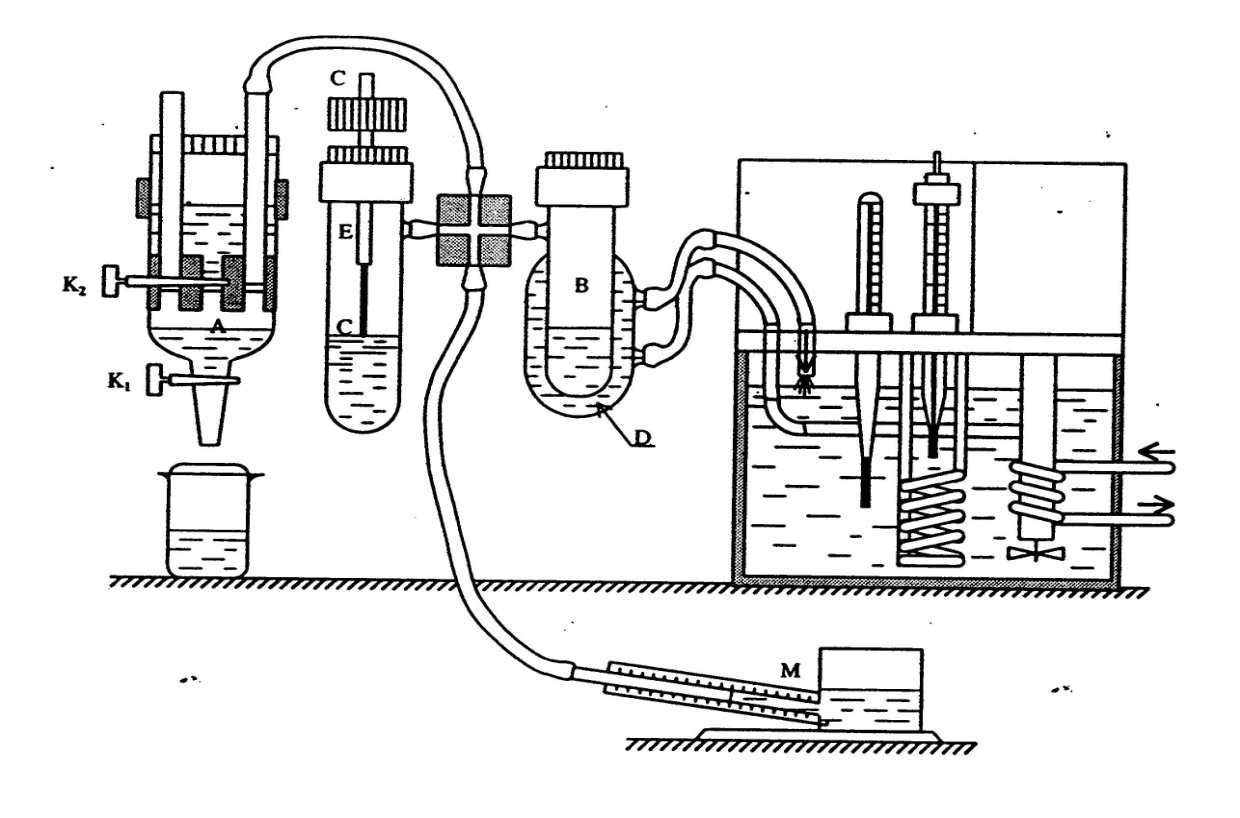
\includegraphics[width=0.7\linewidth]{Scheme}
\label{fig:scheme}			
\end{figure}
		\\
		\\
		Обычно кончик иглы лишь касается поверхности жидкости, чтобы исключить влияние гидростатического давления столба жидкости. Однако при измерении температурной зависимости коэффициента поверхностного натяжения возникает ряд сложностей. Во-первых, большая теплопроводность металлической трубки приводит к тому, что температура на конце трубки заметно ниже, чем в глубине жидкости. Во-вторых, тепловое расширение поднимает уровень жидкости при увеличении температуры.
		\\
		\\
		Обе погрешности можно устранить, погрузив кончик трубки глубже в жидкость. Полное давление, измеренное при этом микроманометром, $P = \Delta P + \rho gh$. $\rho gh$ не зависит от температуры жидкости. Величину $\rho gh$ следует измерить двумя способами. Во-первых, замерить величину $Р1= \Delta P'$, когда кончик трубки только касается поверхности жидкости. Затем при этой же температуре опустить иглу глубже в жидкость и замерить $Р2 = \rho gh + \Delta P"$ ($\Delta P'$, $\Delta P"$ – давление Лапласа). Из-за несжимаемости жидкости можно положить $\Delta P'= \Delta P"$ и тогда $\rho gh = Р2 - Р1$. Во-вторых, при измерениях Р1 и Р2 замерить линейкой глубину погружения иглы h.
		
	\section*{Выполнение работы}

\end{document}